% !TEX root =../LibroTipoETSI.tex
%El anterior comando permite compilar este documento llamando al documento raíz
\chapter{Introducción}\label{chp-01}
\epigraph{All models are wrong, but some are useful}{George Box, 1976}

\lettrine[lraise=-0.1, lines=2, loversize=0.2]{E}{l} interés en los vehículos aéreos no tripulados UAV (\textit{Unmanned Aerial Vehicle}) está en aumento. Dos grandes sectores en el mercado de los UAVs son el de consumo, como aquellos que se usan con fines de ocio, y el comercial, como los que son usados en los negocios o instituciones para realizar algún tipo trabajo. 
Un ejemplo de su aplicación se puede ver en una prueba piloto \cite{telefonica} que consiste en utilizar las torres de comunicaciones para albergar un UAV que se dirige de forma autónoma hasta la zona de un posible incendio, si recibe un aviso de sensores infrarrojos situados en al misma torre de comunicaciones.
\begin{figure}
   %\centering
   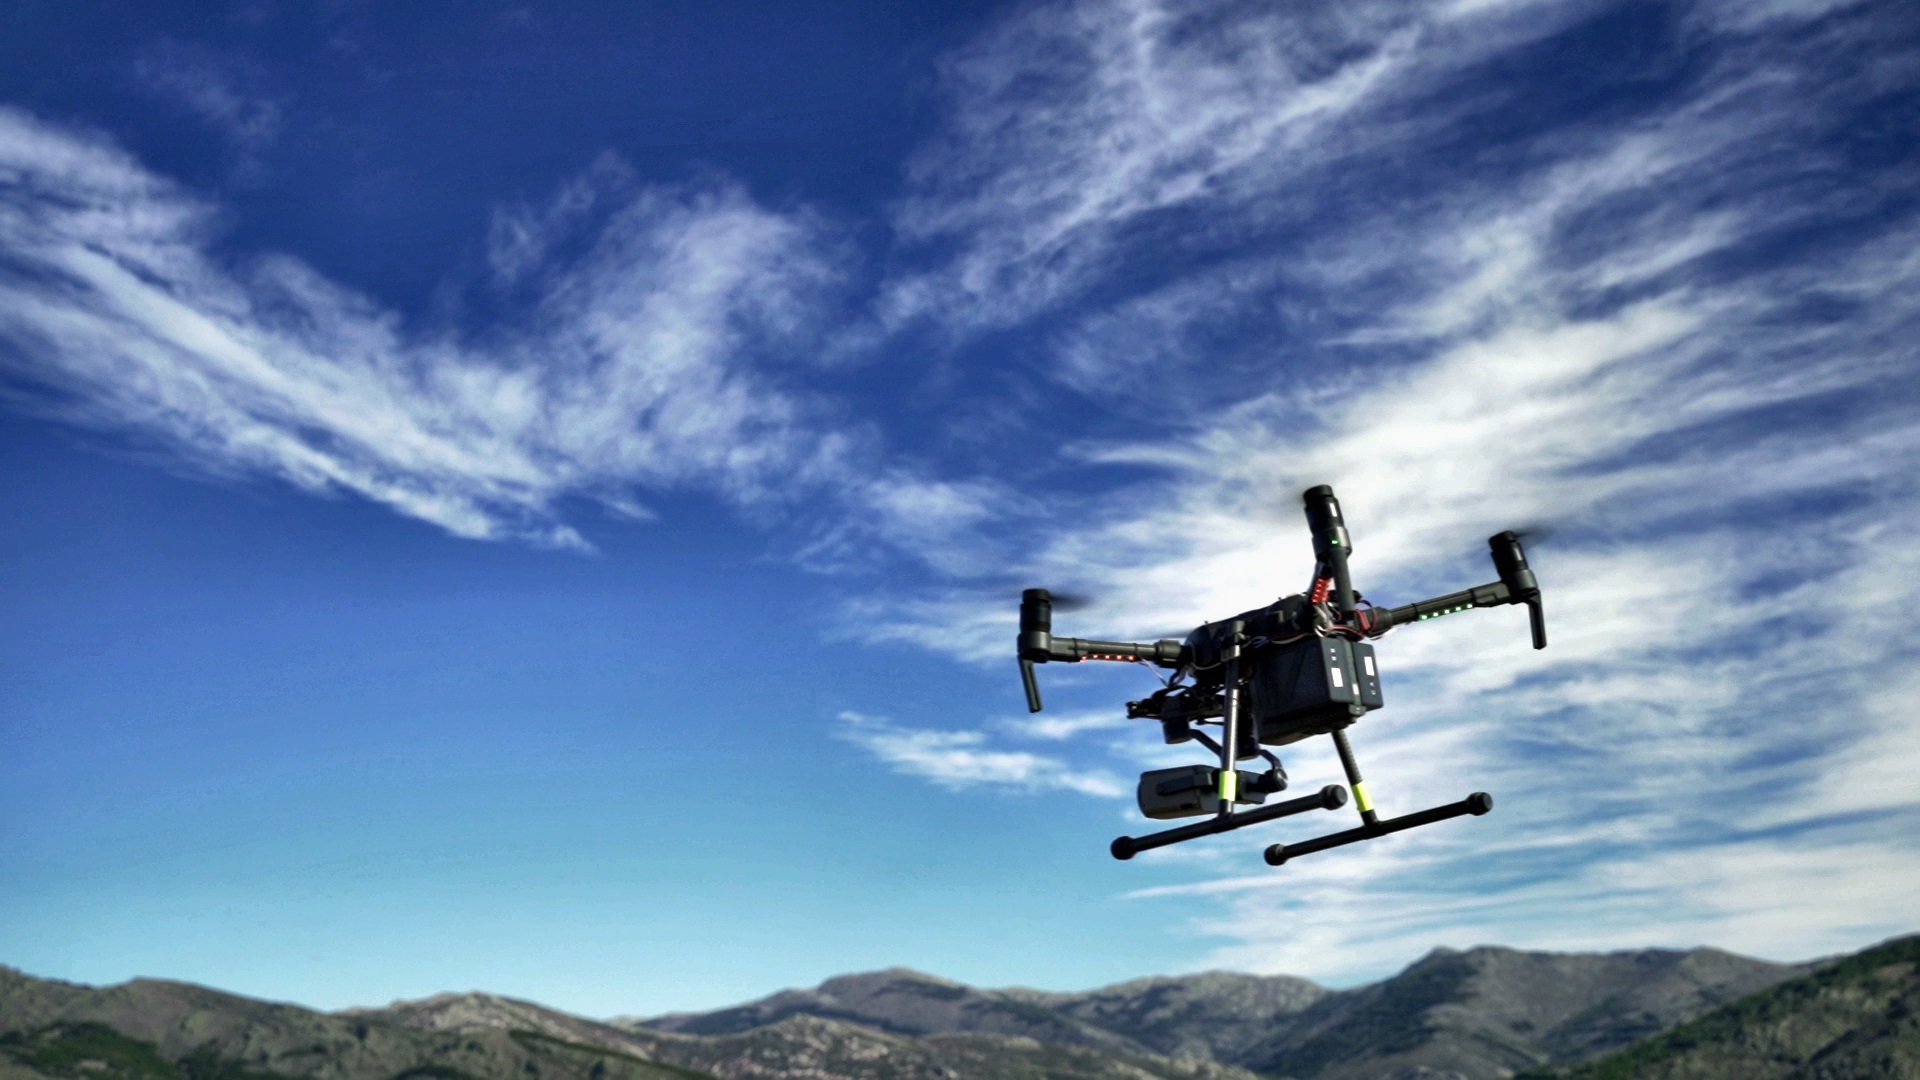
\includegraphics[width=0.3\textwidth]{introduccion/drone-incendio.jpg}\ 
   \caption{Prueba piloto de UAV antiincendios. Fuente \cite{telefonica} }
   \label{fig:telefonica}
\end{figure}

Este último sector es el que se  espera que experimente un mayor aumento y se predice que su tamaño se triplique en el año 2023 \cite{mercado-drones}.
Su crecimiento se ve limitado por diversos factores entre los que destacan las regulaciones, como la necesidad de estar dentro del alcance visual del piloto, o la autonomía de las baterías. Esto último es más notorio en aquellos vehículos de ala rotativa como los helicópteros o quadrotors, ya que son mucho menos eficientes que los de ala fija como los aeroplanos. Sin embargo, tienen mayor maniobrabilidad que estos últimos puesto que, entre otras cosas, son capaces del despegue y aterrizaje en vertical. 

Dadas las ventajas de cada uno de estos tipos nace la idea de \textit{VTOL}, que son los aviones con capacidad de despegue vertical. Un caso de ellos son los tiltrotors, que son aquellos que poseen rotores (también llamados proprotores) que se inclinan. 
En \cite{tiltrotor-review} se hace una recopilación de los estudios sobre diferentes técnicas de control de estos vehículos, tanto de 2, 3 o 4 rotores. Para el caso de 2 rotores, en \cite{tiltrotor-control} y  \cite{tiltrotor-control2} se proponen distintos controladores.  


En este trabajo se diseñará un controlador para el modo helicóptero de un tiltrotor y se implementará en un autopiloto de código abierto llamado \textit{PX4}. Este es un proyecto comenzado en 2009 por la \textit{Escuela Politécnica Federal de Zúrich} (ETH) que ofrece todo el software necesario para hacer que los vehículos aéreos, acuáticos o terrestres naveguen de forma autónoma. 

~\cite{windup}

\endinput
